\section{Replacing the context by a shorter description}
\label{comp:section}

The marking procedure gives useful conditional laws, but the history
producing those laws is too large to retain indefinitely. We now replace
that history by a new message which describes smaller flag domains.
The encoder may use the old history and its conditional laws; the new
decoder must work without them. This distinction is essential to
iterating the construction.

Throughout this section the parameters are those of
\eqref{base:parameters}, and all constants may depend on the fixed
dimension, on \(\eta\), and on fixed constants in the input hypotheses.
In particular, \(q\) may be taken sufficiently large in terms of those
constants.

\begin{lemma}[One compression step]\label{comp:step}
Let \(F\) be a consistent tuple of deterministic length
\(c_0k\le \ell\le k\), for a fixed \(c_0>0\), extracted in one of the two
orientations from the flag stream. Suppose that the stream law is
dominated by a fixed constant times its original independent law and
is supported on the rectangle-occupancy event of
Lemma~\ref{base:rectangles}.
Let a discrete context \(\mathsf C\) specify a domain for each slot, with
\[
 H(\mathsf C)\le\Lambda,\qquad
 |\text{domain of each slot}|\le Cq^d e^\Delta,
 \qquad \Lambda,\Delta\ge0.
\]
Define, as in \eqref{mark:parameters},
\[
 D=\sigma^\beta(1+\Lambda/k+\Delta\sigma^{-\eta}),
 \qquad \sigma^\beta\le D\le\sigma^{1-\eta/2}.
\]
There is an extraction of a consistent tuple \(F'\) of deterministic
length \(\ell'=\Theta(k)\), still in one of the two stream orientations,
and a new discrete context \(\mathsf C'\) for which
\begin{equation}\label{comp:step-bounds}
\begin{split}
 H(\mathsf C')&\le\Lambda'
     \le CqP\log(w+2)(\sigma+wP)+Cw\sigma,\\
 |\text{domain of each slot of }F'|
     &\le Cq^d e^{\Delta'},\qquad
       \Delta'\le CK_*,\\
 &\hspace{1em}1\le w\le C\sigma^{1+\eta/2}/D.
\end{split}
\end{equation}
Here \(w\) is a deterministic integer fixed during the preparation of
the step. The new decoder uses only \(\mathsf C'\), fixed public
parameters, and fixed public tables; it does not use \(\mathsf C\).
The extraction is obtained by conditioning on an event of probability
bounded below by a positive constant. Consequently its stream law
still has constant domination and satisfies the same occupancy bound.
All constants, including the retained proportion, are independent of
\(q\). They and the sufficiently-large-\(q\) threshold are uniform
over the input laws and contexts: they depend only on \(d,\eta,c_0\)
and fixed numerical bounds for the domination constant and the
domain prefactor, not on the realized history or on \(\Lambda,\Delta\)
within the stated admissible range.
\end{lemma}

The preparation in Section~\ref{mark:section} selects a class, an
orientation, equal windows, a pre-round history \(\theta\), and fresh
representative indices. It loses only a fixed proportion of the tuple,
and has the entropy and goodness guarantees in
Lemma~\ref{mark:representatives} and
Proposition~\ref{mark:good-indices}.
We first treat the high-rank classes. For the reciprocal classes we
choose auxiliary supports, use them in a chronological tree of tests,
and finally bound the length of the resulting message. This proves
Lemma~\ref{comp:step} at the end of the section.

\subsection{A bound for unions of rich subspaces}

The rich-subspace viewpoint was motivated by the finite-field
Nikodym maximal estimates of Ellenberg, Oberlin, and
Tao~\cite[Section~4.4, Theorem~4.6]{EOT}.
The precise closure estimate used here is the Nie--Wang inequality
identified below, not an application of those maximal estimates.

The high-rank construction will describe a second point by requiring
its associated subspace to contain many points from a known row.
The following finite-field bound controls the union of all subspaces
that could pass this requirement. It is a consequence of Nie and
Wang's finite-degree closure inequality
\cite[Theorems~4.1 and~5.6]{NieWang2015}. We give a short evaluation-rank
proof to make the precise density dependence available here.

\begin{lemma}\label{comp:rich-union}
Write \(\PG(d,q)=\PG(\F_q^{d+1})\).
Let \(X\subseteq\PG(d,q)\) and \(0<\delta\le1\). Let \(\mathcal V\)
be any family of nonzero vector subspaces of \(\F_q^{d+1}\) satisfying
\[
 |X\cap\PG(V)|\ge\delta|\PG(V)|\qquad(V\in\mathcal V).
\]
Then
\[
 \left|\bigcup_{V\in\mathcal V}\PG(V)\right|
       \le C_d\delta^{-(d+1)}|X|.
\]
\end{lemma}

\begin{proof}
If \(X\) or \(\mathcal V\) is empty, the result is immediate.
Suppose otherwise, and put \(n=d+1\).
Denote by \(\widetilde X\) the set of all nonzero vector
lifts of points of \(X\), and by \(\widetilde Y\) the nonzero vector
points of the union of the spaces in \(\mathcal V\).

We use the Schwartz--Zippel zero bound
\cite{Schwartz1980,Zippel1979}: a nonzero polynomial of total degree
at most \(h\) on \(\F_q^r\) has at most \(hq^{r-1}\) zeros. To see this,
induct on \(r\), writing the polynomial as a polynomial of degree \(t\)
in the last coordinate. Its nonzero leading coefficient has degree
at most \(h-t\) in the other coordinates. There are at most
\((h-t)q^{r-2}\) choices at which that coefficient vanishes; for every
other choice there are at most \(t\) roots in the last coordinate.
The asserted bound follows, with the univariate case starting the
induction.

Fix a sufficiently small constant \(c>0\), and put
\(h=\lfloor c\delta q\rfloor\).
If \(V\) has vector dimension \(r\), at least
\(\delta(q^r-1)\) of its vector points belong to \(\widetilde X\).
This is greater than \(hq^{r-1}\). Thus every polynomial of degree
at most \(h\) vanishing on \(\widetilde X\) vanishes identically on
each such \(V\), and hence on \(\widetilde Y\).
Writing \(\mathrm{ev}_Z\) for evaluation on a set \(Z\), restricted to
these low-degree polynomials, gives
\begin{equation}\label{comp:rich-rank-upper}
 \ker(\mathrm{ev}_{\widetilde X})
       \subseteq\ker(\mathrm{ev}_{\widetilde Y}),
 \qquad
 \operatorname{rank}(\mathrm{ev}_{\widetilde Y})
       \le|\widetilde X|.
\end{equation}

Here is a lower bound for this evaluation rank on an arbitrary
nonempty set \(Z\subseteq\F_q^n\).
The monomials with individual exponents less than \(q\) span all
functions on \(\F_q^n\), by coordinatewise Lagrange interpolation,
so their evaluations on \(Z\) have rank \(|Z|\).
If \(h\ge2n\), partition their exponent box into boxes of side
\(a=\lfloor h/n\rfloor+1\). Every box consists of a fixed monomial
times monomials of total degree at most \(n(a-1)\le h\).
Multiplication by that fixed monomial is a diagonal map on
evaluations, and therefore cannot increase rank. The number of
boxes is at most \(C_d\delta^{-n}\), giving
\[
 \operatorname{rank}(\mathrm{ev}_Z)
       \ge c_d\delta^n|Z|.
\]
Apply this to \(Z=\widetilde Y\), combine with
\eqref{comp:rich-rank-upper}, and divide by \(q-1\).
If \(h<2n\), then \(\delta q\) is bounded in terms of \(d\).
The result instead follows directly from \(|X|\ge1\) and the
ambient bound \(|\PG(d,q)|\le2q^d\), after increasing \(C_d\).
\end{proof}

\subsection{The high-rank classes}

When the early representative is good, we sample both rows from its
conditional flag law restricted to good endpoints. The rows have
different jobs. The first associates a candidate subspace with each
second point. The second tests whether that subspace contains enough
mass of the source's second-endpoint law.
Subspaces with substantial mass have a small union by
Lemma~\ref{comp:rich-union}; the independent second row rarely admits
the remaining candidates. For coverage, consistency will instead show
that the first endpoints of most actual targets annihilate the candidate
subspace. The target law is kept unchanged throughout this comparison.

\begin{lemma}\label{comp:high-rank}
Suppose the preparation in Section~\ref{mark:section} produces a
high-rank class with fixed vector ranks \(r,r'\), where
\(r+r'>d+1\), and one window of length \(\Theta(k)\).
There is a new context of length \(O(q\sigma^{1+\beta})\) bits whose
decoded flag domain has size at most \(q^d e^{O(K)}\).
With probability bounded below, this domain contains a deterministic
number \(\Theta(k)\) of middle targets, retained in their original order.
The decoder does not need the old history or any conditional law.
\end{lemma}

\begin{proof}
Fix the history and fresh indices, and first suppose the early
representative is good. Draw two independent rows, each of
\[
 h=\lceil q\sigma^\beta\rceil
\]
full flags from its conditional marginal conditioned on both
endpoints being good. Write their entries
\((a_t^{(1)},b_t^{(1)})\) and \((a_t^{(2)},b_t^{(2)})\).
These are auxiliary samples, independent of the actual unexposed
tuple given the history and indices. By
\eqref{mark:high-caps} and Lemma~\ref{mark:endpoint-mass},
their first and second marginal atom sizes are at most
\(Ce^K/q^{r'}\) and \(Ce^K/q^r\), respectively, and their
support sizes are at most \(Cq^{r'}\) and \(Cq^r\).

For every second-system projective point \(y\), form the vector space
\[
 V_y=\Span\bigl(y,\ b_t^{(1)}:
                          a_t^{(1)}\perp y,\ 1\le t\le h\bigr).
\]
The decoded domain consists of all flags \((c,y)\) satisfying
\begin{equation}\label{comp:high-domain}
 \dim V_y=r,\qquad c\perp V_y,\qquad
 \#\{t:b_t^{(2)}\subseteq V_y\}\ge .1h/q.
\end{equation}
Here and below, dimensions of the spaces \(V_y\) are vector
dimensions. Because \(y\subseteq V_y\), every pair allowed by
\eqref{comp:high-domain} is indeed an incident flag.

\paragraph{Coverage.}
Consider an actual target at a good middle index, and write it
\((c,y)\). The weighted variance estimate of
Lemma~\ref{base:incidence} shows that, except for at most
\(O(q^{d+1-r'}e^K)\) values of \(y\), a source sample satisfies
\(a\perp y\) with probability at least \(.4/q\).
The mass of these exceptions at a good target endpoint is at most
\[
 Cq^{d+1-r-r'}e^{2K}=o(1).
\]
For a nonexceptional \(y\), while the first-row span has dimension
less than \(r\), it contains at most \(Cq^{r-2}\) second points.
The probability that a sample second endpoint belongs to that span
is at most \(Ce^K/q^2=o(1/q)\). A sample therefore increases the
span with probability at least \(.3/q\) while its rank is too small.
Dividing the row into a fixed number of pieces proves that the
first-row span reaches rank \(r\) with failure probability \(o(1)\).
Independently, the second row has at least \(.1h/q\) first-endpoint
hits on \(y\), again with failure probability \(o(1)\).

Consistency of the actual early representative and target,
Lemma~\ref{base:event-transfer}, and \eqref{mark:good-index} bound
the product-law conflict probability
\(\Prob(a\perp y,\ c\not\perp b)\) by
\(C\sigma^{-2000\beta}/q\).
Conditioning the auxiliary source on good endpoints changes this
by only a constant factor. Across both rows, the probability of
any conflict is at most
\(O(\sigma^{-1999\beta})=o(1)\).
In the absence of a conflict, \(c\) annihilates the span generated by
\(y\) and the second endpoints of all first-endpoint hits in both
rows.

Write \(W_y\) for that combined span. We next bound the joint
event \(\{\dim W_y>r,\ c\perp W_y\}\), without conditioning on
the absence of conflicts or on successful span growth.
Fixing both auxiliary rows leaves the actual target law equal to
its original conditional law \(p_i\): the conditioning on good
endpoints was applied only to the auxiliary source.
Thus the target still has at most
\(Cq^r\) possible second endpoints; for each such \(y\), a
combined span of dimension at least \(r+1\) has at most
\(2q^{d-r-1}\) annihilating first points. Excluding joint atoms
larger than \(e^Kq^{-d}\), their total target probability is
at most \(Ce^K/q=o(1)\). The excluded atom mass is
\(O((\delta_i+1)/K)=o(1)\), by the proof of
Lemma~\ref{mark:endpoint-mass}. If \(r=d\), an excessive span is
the whole vector space and has no projective annihilator.
In particular,
\[
 \Prob(\dim W_y>r,\ c\perp W_y)
 \le \Prob\{p_i(F_i)>e^Kq^{-d}\}+Ce^K/q=o(1).
\]
Thus the first-row and combined spans both have dimension exactly
\(r\), outside an \(o(1)\) exceptional probability. Every
second-row first-endpoint hit then has its second endpoint in
\(V_y\), proving \eqref{comp:high-domain}.

The expected number of bad middle indices is \(o(k)\), as is the
loss from bad target endpoints. A bad early representative can be
declared a failure at cost \(o(1)\). We have therefore proved
coverage of the middle targets with expected loss \(o(k)\).

\paragraph{Size.}
Fix the first row. For every \(y\) with \(\dim V_y=r\), set
\[
 a_y=q\Prob(b\subseteq V_y),
\]
where \((a,b)\) is a further independent sample from the same
source law. Let \(X\) be the source's second-endpoint support.
If \(a_y\ge u>0\), the atom bound implies
\[
 |X\cap\PG(V_y)|\ge c u q^{r-1}e^{-K}.
\]
For \(0<u\le u_0\), with \(u_0>0\) fixed and small, this is
relative density at least \(c u e^{-K}\) in \(\PG(V_y)\).
Since \(y\in\PG(V_y)\), Lemma~\ref{comp:rich-union} gives
\begin{equation}\label{comp:high-tail}
 \#\{y:\dim V_y=r,\ a_y\ge u\}
       \le Cq^r(Ce^K/u)^{d+1}.
\end{equation}
The same bound at \(u=u_0\) accounts for every candidate above
that threshold. On a dyad \(u\le a_y<2u\) below \(u_0\), the
second-row count in \eqref{comp:high-domain} is binomial with
mean at most \(2hu/q\). Its probability of reaching
\(.1h/q\) is at most
\[
 (Cu)^{.1h/q}.
\]
For completeness, put \(t=h/(10q)\) and
\(u_j=u_0\,2^{-j-1}\), \(j\ge0\). If \(C_0\) is the constant
in the binomial bound, the contribution of all these dyads
is at most
\[
 Cq^r e^{(d+1)K}
 \frac{C_0^t(u_0/2)^{\,t-d-1}}
      {1-2^{-(t-d-1)}}.
\]
For large \(q\), \(t\ge d+2\). Choose \(u_0\) so that
\(C_0u_0\le1/2\). The displayed fraction is then bounded
uniformly in \(t\), so no factor exponential in \(h/q\)
remains. Together with the count for \(a_y\ge u_0\),
the expected total number of admitted second points is
at most \(q^r e^{O(K)}\). These dyads cover every arbitrarily
small positive \(a_y\); candidates with \(a_y=0\) never pass.
Markov's inequality gives the same bound, with an enlarged
constant, with high constant probability. Each admitted point
has at most \(2q^{d-r}\) first-point partners, giving the claimed
flag-domain bound.

The decoder receives the two raw rows and \(r\), so the message
length is \(O(h\sigma)=O(q\sigma^{1+\beta})\). Definition
\eqref{comp:high-domain} uses neither \(X\), the probabilities
\(a_y\), nor any other hidden marginal data. The size event and
the event of retaining a prescribed positive fraction of the
middle targets have intersection of probability bounded below.
On that event retain the first prescribed number in order.
\end{proof}

\subsection{Auxiliary supports in a reciprocal class}

We now treat the reciprocal classes. All conditional probabilities
in this subsection are given the history \(\theta\) and the fresh
indices. An auxiliary support is a random set sampled from these
conditional laws, independently of the actual unexposed flags.
The useful property is not merely that this set is large: its
averaged uniform measure must be controlled pointwise.

\begin{lemma}\label{comp:supports}
At every good index in a reciprocal class, there are auxiliary
choices of first and second supports consisting entirely of good
endpoints. If \(A\) is the first support and \(p_i^A\) the
conditional first-endpoint law, then
\begin{equation}\label{comp:support-measure}
 \tfrac12 A_{\max,i}e^{-K}\le |A|\le A_{\max,i},
 \qquad
 \E\frac{\boldsymbol 1_{\{a\in A\}}}{|A|}
       \le C p_i^A(a).
\end{equation}
The analogous assertions hold for the second support \(B\).
All such support choices can be made mutually independently,
conditional on the history and indices.
\end{lemma}

The pointwise inequality is the link to the preceding section: integrating
an incidence indicator against the averaged uniform support measure costs
only a constant relative to the original marginal law. It does not assert
that every chosen pair of supports is sparse. We first transfer incidence
bounds under these independent choices and only later test the realized
supports.

\begin{proof}
Partition each positive marginal support into levels according to
\(\lfloor-\log p\rfloor\). This nonnegative integer has mean at
most the marginal entropy, which is \(O(\sigma)\). Comparison
with a geometric distribution of comparable mean, using
nonnegativity of relative entropy, bounds its entropy by
\(O(\log\sigma)\).

For a pair of level sets \(A_0,B_0\), put
\[
 x=\log(A_{\max,i}/|A_0|),\qquad
 y=\log(B_{\max,i}/|B_0|).
\]
These numbers are nonnegative. The reciprocal caps
\eqref{mark:reciprocal-caps} and incidence mixing give
\[
 e(A_0,B_0)
 \le Cq^d\bigl(e^{-x-y}+e^{-(x+y)/2}\bigr)
 \le C'q^d e^{-(x+y)/2}.
\]
Apply the entropy chain rule to the two level indices and then
bound the conditional flag entropy by the logarithm of this
count. Since \(H_\theta(F_i)=J_0-\delta_i\), this gives
\[
 \E(x+y)\le C(\delta_i+\log\sigma+1).
\]
At a good index, \(\delta_i/K\le\sigma^{-2\beta}\), and
\(\log\sigma=o(K)\). Levels whose loss exceeds \(K\)
therefore carry \(o(1)\) marginal mass.

Within each level the positive weights differ by at most a
factor \(e\). If more than half its points are bad, its bad
points carry at least \(1/(2e)\) of the level's mass.
Equation~\eqref{mark:bad-endpoints} consequently shows that
such levels also carry only \(o(1)\) mass.
Keep the levels with loss at most \(K\) and at least half of
their points good. Choose one with probability proportional
to its original marginal mass, and take its subset of good
points. The size assertion follows immediately.
The retained levels have total mass at least \(1/2\) for
large \(q\). For a point in a retained level, its level mass
divided by the number of good points in that level is at
most \(2e\) times its own mass. The renormalization costs at
most another factor \(2\), proving the pointwise bound.
The same construction applies to the other endpoint and uses
independent auxiliary randomness when desired.
\end{proof}

For brevity put \(\varepsilon=\sigma^{-2000\beta}\).
For good representatives \(i<j\) in distinct representative
blocks, \eqref{mark:incidence-charge},
\eqref{mark:good-index}, and \eqref{comp:support-measure} give
\begin{equation}\label{comp:average-incidence}
 \E\frac{e(A_i,B_j)}{|A_i||B_j|}
       \le C\varepsilon/q.
\end{equation}
Here the two auxiliary support choices are independent.
Their uniform measures vanish outside the good endpoints,
which is precisely the endpoint restriction in the collision
bound. The same argument, using only one auxiliary support,
gives
\begin{equation}\label{comp:target-incidence}
\begin{aligned}
 \E\sum_{a,y}
 \frac{\boldsymbol 1_{\{a\in A_i\}}}{|A_i|}
 p_t^B(y)\boldsymbol 1_{\{y\ {\rm good}\}}
 \boldsymbol 1_{\{a\perp y\}}&\le C\varepsilon/q
       &&(i<t),\\
 \E\sum_{a,y}
 p_t^A(a)\boldsymbol 1_{\{a\ {\rm good}\}}
 \frac{\boldsymbol 1_{\{y\in B_j\}}}{|B_j|}
 \boldsymbol 1_{\{a\perp y\}}&\le C\varepsilon/q
       &&(t<j),
\end{aligned}
\end{equation}
whenever \(t\) is a good middle target and the representative
in question belongs to its fresh representative list.

These incidence bounds also control the chronological movement
of the reciprocal parameter \(u\).
For good representatives \(i<j\) in distinct blocks,
\begin{equation}\label{comp:order}
 u_j\le u_i+CK.
\end{equation}
Indeed, if the difference exceeded a sufficiently large
multiple of \(K\), the lower support sizes in
\eqref{comp:support-measure} and the reciprocal cap formulas
would give
\[
 |A_i||B_j|\ge c q^{d+1}
                    \exp(u_j-u_i-2K)\gg q^{d+1}
\]
for every support choice. Mixing would force incidence
density at least \(c/q\), contradicting
\eqref{comp:average-incidence}.

Delete a window if either representative is bad.
The expected number deleted is \(o(w)\), by
Proposition~\ref{mark:good-indices}.
In an open band, additionally delete a window if
\(u_{\rm early}-u_{\rm late}>K_*\).
Before this additional deletion, the total downward movement
in the chronological list of retained representatives is at
most
\[
 C\sigma+CKw.
\]
To justify this, its total upward movement is at most \(CK\)
per step by \eqref{comp:order}, while all \(u\)'s lie in an
interval of length \(O(\sigma)\).
The additional deletions therefore number at most
\[
 C(\sigma+Kw)/K_*=o(w),
\]
because in an open band
\(w\asymp\sigma^{1+\eta/2}/D\), so
\(\sigma/(wK_*)=O(\sigma^{-\eta/2-6\beta})\) and
\(K/K_*=\sigma^{-3\beta}\).
In an integer band there is no additional deletion:
the two parameters already differ by at most \(2K_*\).

For each remaining window choose \(A\) at the early
representative and \(B\) at the late representative, using
Lemma~\ref{comp:supports}.
Make all these choices independently, and independently of
the remaining flags given the history and fresh indices.
Every resulting pair satisfies
\begin{equation}\label{comp:product}
 |A||B|\ge q^{d+1}e^{-CK_*}.
\end{equation}
Both \eqref{comp:average-incidence} and
\eqref{comp:target-incidence} apply to the corresponding
supports, including those in the same window.
These are averages under the original independent support
choices, before any further support-dependent selection.

\subsection{A chronological tree of fresh tests}

At this point the surviving list of windows is fixed by the
history and fresh indices, before the auxiliary supports are
chosen. If it is empty we declare failure.
Otherwise build the balanced binary search tree on this list:
the middle window is the root, and the earlier and later
halves are treated recursively. Its depth is at most
\(C\log(w+2)\), where \(w\) is the original number of windows.
Every node has inherited first and second point domains,
denoted \(U_A,U_B\); initially both are full projective spaces.

At a pivot with original auxiliary supports \(A,B\), form the
trimmed supports
\[
 S=A\cap U_A,\qquad T=B\cap U_B.
\]
If either size is less than \(.9\) of its original support,
or if
\[
 \frac{e(A,B)}{|A||B|}
       >\frac{\sigma^{-1000\beta}}q,
\]
delete the whole subtree. Otherwise put
\(n_A=|S|\), \(n_B=|T|\) and
\[
 d_A=\log(|U_A|/n_A),\qquad
 d_B=\log(|U_B|/n_B).
\]
The pair \(S,T\) satisfies the hypotheses of
Lemma~\ref{geom:description}: by \eqref{comp:product} its
product is at least \(q^{d+1}e^{-CK_*}\), and its incidence
density is at most \(C\sigma^{-1000\beta}/q\).
Orient the description toward its smaller side and use
Lemma~\ref{geom:validation} to produce both caps, denoted
\(U_A',U_B'\). If any part fails, delete the subtree.
A successful pivot uses both caps for its own targets.
Its left child inherits \((U_A',U_B)\), and its right child
inherits \((U_A,U_B')\).

\begin{figure}[tb]
\centering
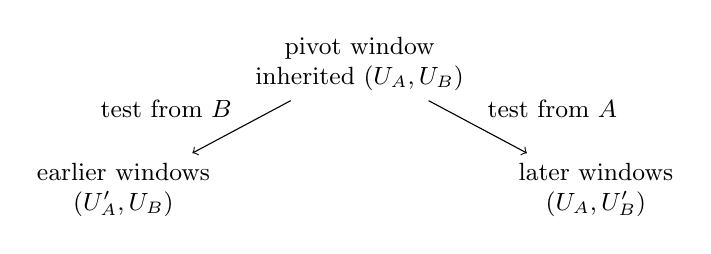
\begin{tikzpicture}[every node/.style={align=center,font=\small}]
 \node (pivot) at (0,0) {pivot window\\inherited \((U_A,U_B)\)};
 \node (left) at (-3,-1.6) {earlier windows\\\((U_A',U_B)\)};
 \node (right) at (3,-1.6) {later windows\\\((U_A,U_B')\)};
 \draw[->] (pivot) -- node[above left] {test from \(B\)} (left);
 \draw[->] (pivot) -- node[above right] {test from \(A\)} (right);
\end{tikzpicture}
\caption{A pivot restricts the first points to its left and
the second points to its right. Its own targets use both
new caps. This is exactly the time direction in
\eqref{comp:average-incidence} and
\eqref{comp:target-incidence}.}
\label{comp:tree-figure}
\end{figure}

All calls use fresh independent public tables. Their
acceptance predicates are exactly those prescribed in
Lemmas~\ref{geom:description} and \ref{geom:validation},
applied to the trimmed inputs \(S,T\) and the captured
subsets produced by those lemmas. These inputs are
determined by the original auxiliary supports, the
history and indices, and earlier auxiliary tables.
Conditional marginal laws are used to choose the original
supports, not as an additional acceptance filter.
No call inspects actual unexposed flags. Thus, given the
history and indices, the entire auxiliary construction
remains independent of those flags. In the loss estimates
below, we compare each test's hidden source with its
original pivot support, which still supplies the
unconditioned incidence bounds.

\begin{lemma}\label{comp:tree-loss}
The expected number of middle targets lost through the
pre-tree deletions, deleted subtrees, or exclusion by the
produced caps is \(o(k)\). In particular, a prescribed
deterministic number \(\Theta(k)\) of targets can be retained in order
with probability bounded below.
\end{lemma}

\begin{proof}
The pre-tree deletions have already been bounded, and all
windows have equal size. It remains to analyze the tests
without conditioning on the later retention of a window.

Fix the history, indices, all original support choices,
and any earlier auxiliary data making a validation test
ready. In the first validation test the hidden source is
the intersection of the described set with one trimmed
support. Description capture and the \(.9\) trim make it
a fixed positive fraction of the corresponding original
support. If this test succeeds, the second test's hidden
source is also a fixed positive fraction of its original
support, by the \(.99\) capture assertion of
Lemma~\ref{geom:validation}.
For either test and every fixed opposite point \(y\), let
\(E_y\) be the event that the test is produced and excludes
\(y\) by its ambient test.
Lemma~\ref{geom:produced-test} gives
\begin{equation}\label{comp:pointwise-test}
 \Prob(E_y\mid\text{readiness data})
       \le Cq\frac{|X\cap N(y)|}{|X|},
\end{equation}
where \(X\) is that test's original pivot support.
The right side no longer depends on the readiness data.
The contribution is zero if the node is not reached or
the test is not ready. We may consequently average over
all earlier auxiliary data with no additional conditioning.

More explicitly, fix one ancestor test and a descendant's
corresponding original support \(Y\). Let \(L\) be the
fraction of \(Y\) excluded by that test, set to zero when
the test is not produced. If \(\mathcal H\) denotes the
history and indices, and \(\mathcal S\) all original support
choices, averaging over readiness data gives
\[
 \E(L\mid\mathcal H,\mathcal S)
       \le Cq\frac{e(X,Y)}{|X||Y|}.
\]
This bound is not conditioned on reaching the test.
Now average the original support choices under their
original independent law.
The chronological inheritance rule ensures that the pair
is always an earlier first support against a later second
support. Equation~\eqref{comp:average-incidence} bounds the
expected lost fraction by \(C\varepsilon\) per ancestor
test. This remains true when readiness data or the
prescribed acceptance predicates depend on other original
support sets: those sets were fixed before
\eqref{comp:pointwise-test} was applied.

At a node of depth \(j\), failure of a trim after all
previous successes requires loss of at least one tenth
of an original support to its ancestor tests. The joint
probability of this event and reaching the node is
therefore at most \(Cj\varepsilon\).
By \eqref{comp:average-incidence} and Markov's inequality,
the unconditional same-node density rejection probability
is at most \(C\sigma^{-1000\beta}\).
Conditional on reaching a ready node, a description or
validation failure costs \(Ce^{-cq}\), uniformly in its
input data. Hence, if \(H=C\log(w+2)\), a fixed window's
probability of deletion somewhere along its path is at
most
\begin{equation}\label{comp:subtree-loss}
 C\varepsilon H^2+
 C\sigma^{-1000\beta}H+Ce^{-cq}H=o(1).
\end{equation}

For an actual good middle target, instead integrate
\eqref{comp:pointwise-test} against its unnormalized good
endpoint mass. Independence of the auxiliary construction
from actual unexposed flags and
\eqref{comp:target-incidence} give an exclusion probability
at most \(C\varepsilon\) per relevant ancestor test.
Both tests are relevant at the target's own pivot.
This count includes a first test as soon as it is
produced, even if the second test subsequently fails.
Neither this estimate nor \eqref{comp:subtree-loss}
conditions on eventual survival of a descendant or target.

The expected bad-index fraction tends to zero by
Proposition~\ref{mark:good-indices}, and the bad-endpoint
mass at every good index tends uniformly to zero by
Lemma~\ref{mark:endpoint-mass}.
Combining these losses with \eqref{comp:subtree-loss}
and the \(O(H)\) relevant tests gives expected total
loss \(o(k)\).
The original middle-target population is a fixed positive
multiple of \(k\). With probability tending to one,
at least a prescribed smaller positive multiple remains;
retain the first prescribed number in order.
\end{proof}

\subsection{The new decoder and its message length}

The loss argument has shown that many targets survive.
We must now verify that their domains can be reconstructed
from the new message alone, and that the message has the
bound asserted in Lemma~\ref{comp:step}.

The message specifies the surviving-list tree, construction
statuses, all successful node descriptions and validation
messages, the necessary support sizes and orientations,
and the number of retained targets at each pivot.
These additional discrete data cost \(O(w\sigma)\) bits.
In particular, original slot labels are not sent.
Traversing the tree in chronological order and using the
retained counts specifies the domain of each new tuple
slot.

The decoder starts with full point domains, prescribed
public parameters, and a fresh table address for every
call at every tree address. It reconstructs the domains
recursively from successful messages.
At each successful node its header supplies \(n_A,n_B\)
and the orientation and mode choices. The inherited domains
then determine \(d_A,d_B\). In particular, the validation
row lengths \(\lceil C_0q(d_A+1)\rceil\) and
\(\lceil C_0q(d_B+1)\rceil\), and the associated finite search
cutoffs, are determined from these data and public constants.
Any other row-length diagnostics required inside a
description are sent within that lemma's message budget.
Table addresses consist of the binary tree word, the call
phase (description, first validation, or second validation),
and the internal call address used by that subroutine.
Thus neither the table choice nor a variable row length
requires the old history.
An acceptance predicate can involve a hidden support,
but the accepted proposal row is recoverable from its
transmitted index without checking that predicate again.
A failed construction deletes its whole subtree; no
retained descendant depends on a failed test that was
not transmitted. This also explains why descriptions
of failed constructions need not be part of the message.
None of this reconstruction uses the old context,
conditional laws, or hidden support sets.

At a successful node, validation gives
\[
 |U_A'|\le Cq^{d+1}/n_B,\qquad
 |U_B'|\le Cq^{d+1}/n_A.
\]
Since \(n_An_B\ge q^{d+1}e^{-CK_*}\), mixing between
the two caps gives at most
\begin{equation}\label{comp:new-domain}
 Cq^d e^{CK_*}
\end{equation}
incident flags in their product. This is the domain
assigned to each retained target at that pivot.

An independent ambient-size bound at each node would charge
\(O(\sigma)\) at every pivot. Instead, the two children
jointly receive the parent's two marginal gaps, up to
\(O(K_*)\). We use this additive bound to sum the costs
level by level. Put
\[
 G=\log(|U_A||U_B|/q^{d+1})
\]
at a node with nonempty data. Its support gaps obey
\begin{equation}\label{comp:gap-potential}
 d_A+d_B\le G+CK_*.
\end{equation}
The description and validation together cost
\(O(qP(d_A+d_B+P))\).
For a successful node the children satisfy
\[
 G_{\rm left}^+\le d_B+C,\qquad
 G_{\rm right}^+\le d_A+C,
 \qquad x^+=\max(x,0).
\]
Indeed the left child inherits \(U_A',U_B\), so its
untruncated potential is at most
\(\log(C|U_B|/n_B)=d_B+C\); the other child is symmetric.
It follows from \eqref{comp:gap-potential} that
\begin{equation}\label{comp:potential-branch}
 G_{\rm left}^++G_{\rm right}^+
       \le G^++CK_*.
\end{equation}
The root potential is \(O(\sigma)\).
Pruning can only reduce a positive-potential sum, and
charging \eqref{comp:potential-branch} to the at most
\(w\) ancestors shows that the sum of positive
potentials at any level is at most
\(C(\sigma+wK_*)\).
There are \(O(\log(w+2))\) levels. Summing the successful
node costs, using \(K_*=o(P)\), and including the
additional discrete data gives the deterministic bound
\begin{equation}\label{comp:tree-cost}
 CqP\log(w+2)(\sigma+wP)+Cw\sigma.
\end{equation}
All row searches have the prescribed finite cutoffs of
the description and validation lemmas, so this is a
maximum message-length bound, not only an expected one.
Self-delimiting messages convert it to the same entropy
bound after an absolute constant adjustment.

\begin{proof}[Proof of Lemma~\ref{comp:step}]
Apply the preparation of Section~\ref{mark:section}.
Its class selection conditions on an event of probability
bounded below; its choices and orientation are determined
by the revealed history. In a high-rank class use
Lemma~\ref{comp:high-rank}, with \(w=1\).
Its cost \(O(q\sigma^{1+\beta})\) is bounded by
\eqref{comp:step-bounds}, and its exponent \(O(K)\)
is \(O(K_*)\).
In a reciprocal class use the support construction,
tree, and Lemma~\ref{comp:tree-loss}.
Equations~\eqref{comp:new-domain} and
\eqref{comp:tree-cost} give the required output budgets.
The window sizes in \eqref{mark:windows} imply
\[
 w\le C\sigma^{1+\eta/2}/D
\]
in both reciprocal cases, and this bound also holds
for \(w=1\) under the admissible range of \(D\).

Initially average over the fresh public tables as well
as the auxiliary support choices and other randomness.
The preceding arguments give a probability bounded
below of having the required number of targets and
all asserted output properties. Hence some fixed
choice of the entire public table family retains a
bounded-below probability of this event. Fix that
family first, then condition on successful extraction
of the prescribed deterministic length.
The fresh table family was independent of the input stream,
so fixing it does not change the input stream's marginal law.
For any stream event, the subsequent success conditioning increases its
probability by at most the reciprocal of the fixed
success probability. Thus constant domination
persists, while the occupancy property persists
pointwise. The retained tuple is an ordered subtuple
in the selected orientation and remains consistent.

The message-length and domain bounds hold for every
successful history and every fixed table realization,
not merely on average over histories. They therefore
remain valid under this possibly biased conditioning.
The new context is precisely its standalone message,
not that message together with the old history.
Consequently its entropy and slot domains satisfy
\eqref{comp:step-bounds}, with fixed constants, as
asserted.
\end{proof}
